\section{Literatür Taraması}

\subsection{Çoklu Ajanlı Yol Bulma (MAPF) Problemi}

Endüstri 4.0'ın gelişimi ve otonom depo sistemlerinin yaygınlaşmasıyla birlikte, Otonom Yönlendirmeli Araçların (AGV) paylaşımlı alanlarda eş güdümlü hareketi literatürde büyük bir ivme kazanmıştır \citep{WUReview2023}. Standart MAPF problemi (\textit{Multi-agent Pathfinding}), etkenlerin birbirleriyle çarpışmadan, kilitlenme (\textit{deadlock}) yaşamadan başlangıç noktalarından hedeflerine ulaşmalarını amaçlar. Ancak bu etkenlerin güzergahlarının, uzay ve zaman kısıtları altında optimal bir biçimde hesaplanması, problemi hesaplamasal olarak oldukça zorlayıcı (\textit{genellikle NP-Zor}) bir yapıya dönüştürmektedir \citep{SURYNEKProblem2022a}.

\subsection{MAPF Çözüm Yaklaşımları}

Literatürdeki MAPF çözümleri genel olarak Bütüncül (\textit{Centralized/Optimal}) ve Ayrık (\textit{Decoupled/Suboptimal}) algoritmalar olmak üzere çeşitli dallara ayrılmaktadır. Çatışma Tabanlı Arama (\textit{Conflict-Based Search - CBS}) veya MILP/SAT tabanlı derleme yöntemleri teorik olarak optimal çözümler sunsa da, sistemdeki araç sayısı arttıkça hesaplama maliyetleri gerçek zamanlı uygulanabilirliği imkansız hale getirebilmektedir \citep{SURYNEKProblem2022a}. Bu nedenle endüstriyel ve dinamik AGV navigasyonunda hız, ölçeklenebilirlik ve pratikliği bir araya getiren Öncelik Tabanlı (\textit{Priority-Based}) ve Kural Tabanlı (\textit{Rule-Based}) yaklaşımlar daha sık tercih edilmektedir \citep{WUReview2023}. Öğrenme tabanlı yaklaşımlar literatürde yer bulmaya başlasa da, bu yöntemler henüz gerçek saha dağıtımlarından ve kesin kural doğrulamasından uzak kabul edilmektedir.

\subsection{Öncelikli Planlama ve Cooperative A*}

Öncelik tabanlı planlamanın temel taşlarından biri, David Silver tarafından literatüre kazandırılan  İşbirlikçi Yol Bulma (\textit{Cooperative Pathfinding}) ve buna bağlı Cooperative A* (CA*) algoritmasıdır \citep{SILVERCooperative2005}. Ayrık bir çözüm sunan CA*, etkenlerin harita üzerindeki hareketlerini eş güdümle hale getirmek için zaman boyutunu da içeren bir Uzay-Zaman Yer Ayırma Tablosu (\textit{Space-Time Reservation Table}) kullanır. Bu mimaride, etkenlere belirli bir öncelik sırası atanır. Her etken, uzay-zaman matrisinde kendi güzergahını bulurken, kendinden daha yüksek öncelikli etkenlerin belirli bir $t$-anında ayırttığı konum düğümlerinden kaçınır. Bu sayede dinamik engellerden kaçınma işlemi, üç boyutlu $(x, y, t)$ bir yol arama problemine indirgenmiş olur.

\subsection{Önerilen Değişiklik}

Orijinal CA* algoritması geniş ızgara (grid) tabanlı haritalarda başarılı sonuçlar verse de, dar koridorlar ve tek şeritli endüstriyel topolojilerde iki temel zafiyete sahiptir: (i) Eşit öncelikli etkenlerin çizelgeleme sırasının çözüme etkisi ve (ii) dar alanlarda kaçacak yer bulamayan etkenlerin oluşturduğu \autoref{fig:literatür-corridor-deadlock}'deki koridor kilitlenmeleri (\textit{corridor deadlocks}) (\cite{SILVERCooperative2005}). Literatürdeki derleme tabanlı veya bütüncül çözümler bu kilitlenmeleri aşabilse de hesaplama maliyetleri AGV sistemleri için çok yüksektir (\cite{SURYNEKProblem2022a}).

\begin{figure}[h!]
    \centering
    %   \fbox{\rule{0pt}{4cm}\rule{0.7\linewidth}{0pt}}
    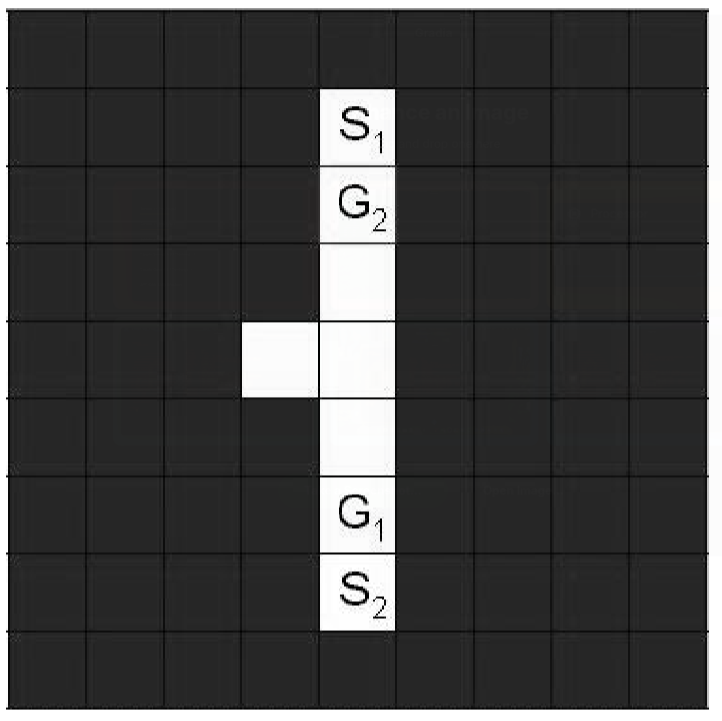
\includegraphics[width=0.5\linewidth]{img/corridor-deadlock.png}
    \captionsetup{width=0.6\linewidth, justification=justified} % Görsel genişliğinin %80'ine sığdırır ve iki yana yaslar
    \caption{Bu basit problem CA* ile çözülememektedir. \protect\ Bir etken S1'den G1'e yol alması gerekirken  diğeri \protect\ S2'den G2'ye hareket etmeye çalışmaktadır. \citep{SILVERCooperative2005}}
    \label{fig:literatür-corridor-deadlock}
\end{figure}

Bu çalışmada, tek şeritli yol yapısının getirdiği kısıtlar doğrultusunda klasik CA* algoritması üzerinde dört aşamalı, özgün bir melez (kural ve öncelik tabanlı) değişiklikler gerçeklenmiştir:

\begin{itemize}
    \item \textbf{Çizelgeleme ve Gecikmeli Çıkış Mekanizması:} Klasik algoritmalardaki rastgele veya statik sıralama yerine; araçların özel öncelik durumunu ($1-v_i$), yolun ilerisindeki araçların trafiği önce boşaltması amacıyla başlangıç konumunu ($-x_{\text{başlangıç}, i}$), hedefe kalan mesafelerini ($d_i$) ve toplam görev yüklerini ($-W_i$) kapsayan dört bileşenli bir sözlüksel öncelik vektörü $\rho_i = (1-v_i, -x_{\text{başlangıç}, i}, d_i, -W_i)$ (\autoref{sec:önceliklendirme-ve-kilitlenme-çözümü}) tanımlanmıştır. Ayrıca, uzay-zaman matrisinin yoğunluğundan kaynaklanan yapay kilitlenmeleri (artificial deadlock) engellemek adına, geçerli rota bulamayan araçların sisteme giriş anı ($t_{\text{başlangıç}}$) dinamik olarak ötelenmiştir (Delayed Release). Bu sayede sisteme araç enjeksiyonu optimize edilmiştir.
    \item \textbf{Yolda Bekleme Yasağı:} Olası fiziksel zıt yön çatışmalarını engellemek adına, araçların ana transit yol üzerinde durarak bekleme yapması (\textit{wait action}) tamamen yasaklanmıştır. Tüm durma ve yol verme eylemleri, kapasite kısıtlı cepler ($C$) ve ara depolar ($G$) ile sınırlandırılmıştır (\autoref{sec:sistem-kısıtları}).
    \item \textbf{Asimetrik Maliyet Fonksiyonu:} Algoritmanın araçları rotayı uzatan gereksiz çık-dön (\textit{yo-yo}) manevralarından kaçındırması adına asimetrik bir maliyet yapısı kurgulanmıştır (\autoref{sec:maliyet-fonksiyonu}). Hareket eyleminin maliyeti $1.0$ olarak belirlenirken, güvenli alanlarda (cep, depo, başlangıç) bekleme maliyeti $0.9$ olarak atanmıştır. Bu ağırlıklandırma, araçların ana yolu işgal etmek yerine matematiksel olarak güvenli noktalarda duraklamasını teşvik etmektedir.
    \item \textbf{Araç İçi Görev Sıralaması (SJF):} Çoklu depo ziyareti gerçekleştirecek araçların kendi içindeki görev rotaları, En Kısa İş İlk (\textit{Shortest Job First}) yaklaşımıyla optimize edilmiştir (\autoref{sec:araç-içi-görev-sıralaması}). Depolar başlangıç noktasına olan mutlak uzaklıklarına göre yakından uzağa sıralanarak, kısa mesafeli görevlerin hızla bitirilmesi, ana yolun erken boşaltılması ve uzay-zaman matrisindeki rezervasyon çakışmalarının minimize edilmesi sağlanmıştır.
\end{itemize}

Önerilen bu dinamik çizelgeleme, asimetrik maliyet yönetimi ve alana özgü kısıt tümleştirmesi, MAPF literatüründeki dar koridor kilitlenmesi problemini bu projenin kısıtları dahilinde deterministik ve düşük bir hesaplama maliyetiyle çözüme kavuşturmuştur.
